\documentclass[crop,class=article]{standalone}
%----------------------------Preamble-------------------------------%
\usepackage{tikz}                       % Drawing/graphing tools.
\usetikzlibrary{arrows.meta}            % Latex and Stealth arrows.
%--------------------------Main Document----------------------------%
\begin{document}
    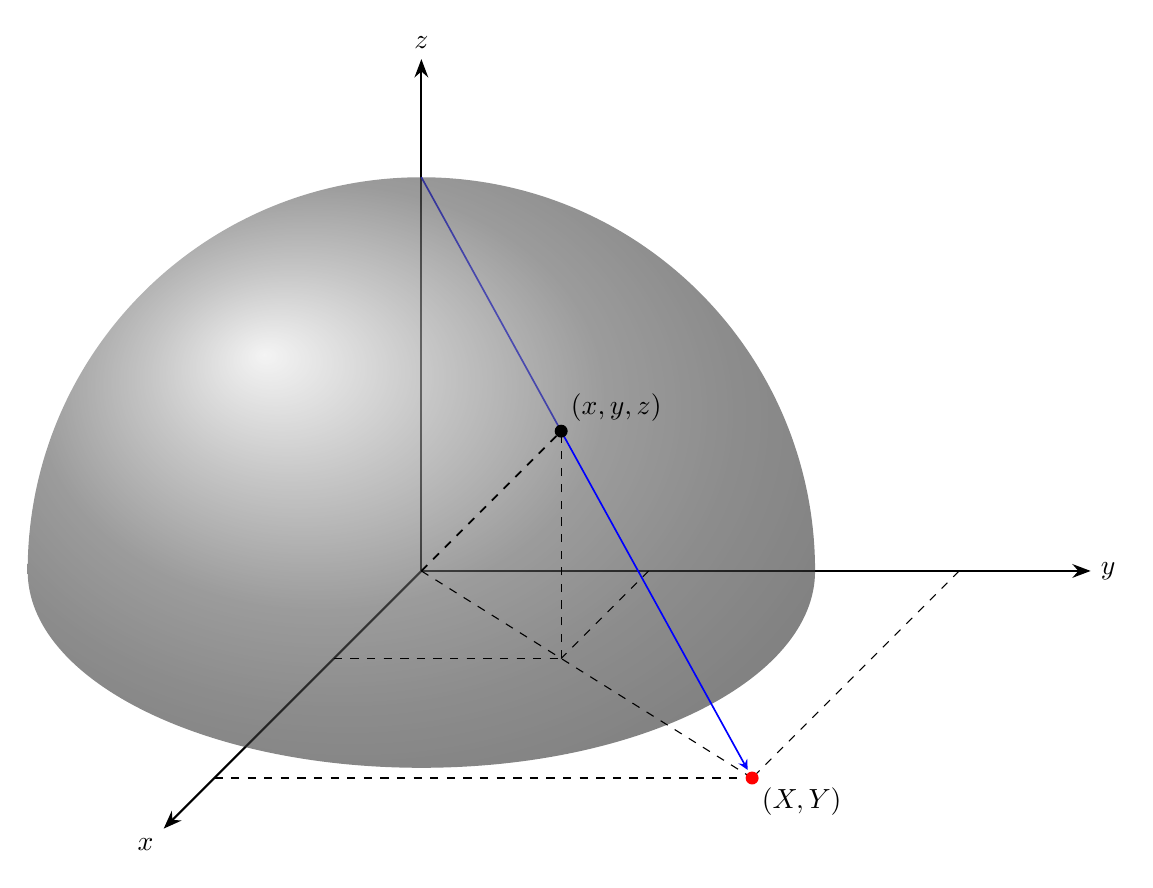
\begin{tikzpicture}[scale=5, >=Stealth]
        % Draw the main coordinate system axes
        \draw[thick,->] (0,0,0)--(1.7,0,0) node[right] {$y$};
        \draw[thick,->] (0,0,0)--(0,1.3,0) node[above]{$z$};
        \draw[thick,->] (0,0,0)--(0,0,1.7) node[below left]{$x$};

        % The point (x,y,z)
        \coordinate (A) at (0.577350269,0.577350269,0.577350269);

        % The projection point (X,Y)
        \node[circle, inner sep=0pt, outer sep=1mm]
            (B) at (1.3660254,0,1.3660254) {};

        % Draw blue line "inside" sphere.
        \draw[draw=blue,semithick] (0,1,0) -- (A);

        % Draw sphere.
        \shade[ball color=gray, opacity=0.6]
            (1cm,0) arc (0:-180:1cm and 5mm)
            arc (180:0:1cm and 1cm);
        
        % Draw blue line "outside" of sphere.
        \draw[draw=blue, semithick, >=stealth, ->] (A)--(B);

        % Draw projection lines.
        \begin{scope}[every path/.style={dashed,thin}]
            \path (0,0,0) edge (1.3660254,0,1.3660254);
            \path (0,0,1.3660254) edge (1.3660254,0,1.3660254);
            \path (1.3660254,0,0) edge (1.3660254,0,1.3660254);
            \path (0,0,0.5774) edge (0.5774,0,0.5774);
            \path (0.5774,0,0) edge (0.5774,0,0.5774);
            \path (0.5774,0,0.5774) edge (0.5774,0.5774,0.5774);
            \path (0,0,0.5774) edge (0.5774,0,0.5774);
        \end{scope}

        % Draw the position vector.
        \draw[dashed,semithick] (0,0,0) -- (0.5774,0.5774,0.5774);

        \filldraw[black] (0.57735,0.57735,0.57735) circle (0.15mm);
        \filldraw[red] (1.3660254,0,1.3660254) circle (0.15mm);
        \node at (A) [above right] {$(x,y,z)$};
        \node at (B) [below right] {$(X,Y)$};
    \end{tikzpicture}
\end{document}